\documentclass[12pt, openany]{book}
\usepackage[letterpaper, margin=1in]{geometry}
\usepackage{setspace}
\usepackage[utf8]{inputenc}

% By default, LaTeX doesn't indent the first line in a paragraph
\usepackage{indentfirst}

% Load images
\usepackage{graphicx}
\graphicspath{ {./images/} }

\usepackage[hidelinks]{hyperref}

% APA citations and bibliography
\usepackage{apacite}

\setlength\parindent{1cm}
\doublespacing

\raggedbottom

\makeatletter
\renewcommand*\@makechapterhead[1]{%
   %\vspace*{50\p@}%
   {\parindent \z@ \raggedright \normalfont
     \ifnum \c@secnumdepth >\m@ne
         \huge\bfseries \@chapapp\space \thechapter
         \par\nobreak
         \vskip 20\p@
     \fi
     \interlinepenalty\@M
     \Huge \bfseries #1\par\nobreak
     \vskip 40\p@
   }}
\renewcommand*\@makeschapterhead[1]{%
   %\vspace*{50\p@}%
   {\parindent \z@ \raggedright
     \normalfont
     \interlinepenalty\@M
     \Huge \bfseries  #1\par\nobreak
     \vskip 40\p@
   }}
\makeatother

% Reset page numbering as book format places them at the top.
\pagestyle{plain}

% Use Helvetica since it's the closest font to Arial
\usepackage{helvet}
\renewcommand\familydefault{\sfdefault}

\begin{document}

\frontmatter
\begin{titlepage}
    \begin{center}
        \vspace{6em}

        
\includegraphics[scale=0.25]{logo.png}

        \begingroup
        % \fontsize{14pt}\selectfont
        \textbf{
            \uppercase{Preventing Academic Malpractice During Online Examinations using Machine Learning}
        }
        \endgroup

        \vspace{6em}

        \textbf{A Thesis\\
            Presented to the Faculty of AMA Computer College}

        \vspace{6em}

        In Partial Fulfillment of the Requirements for the Degree\\
        Bachelor of Computer Science

        \vspace{5em}

        by

        \vspace{3em}

        \textbf{
            Joshua Timothy Abad \\
            Chrisia Bernardo \\
            Kevin Mckhaey Dabu \\
            Rhycca Mae Gutierrez \\
            Greek Genver Legaspi
        }

        \vspace{2em}

        Month 2021

    \end{center}
\end{titlepage}

\section*{\hfill Approval Sheet \hfill}

In partial fulfillment of the requirements for the College department of \textbf{BSCS}, this entitled \textbf{"\projectName: Preventing Academic Malpractice During Online Examinations using Machine Learning} has been examined and is recommended for acceptance and approval for Oral Defense.

\vspace{2em}

\begin{flushright}
    \uppercase{Ronaldo P. Zurbano, MBA}

    Adviser
\end{flushright}

\vspace{2em}

\subsection*{\centering PANEL OF EXAMINERS}

Approved in partial fulfillment of the requirements for CS Design Project with the grade of \makebox[1.0in]{\hrulefill}.

\vspace{2em}

\begin{center}
    \uppercase{Dr. John Doe}

    Chairman
\end{center}

\vspace{2em}

\noindent \uppercase{Skypes Included, PhD} \hfill \uppercase{Heynong Man}

\noindent Member of the Panelist \hfill Member of the Panelist

\section*{\centering Acknowledgement}

We would like to express our deepest appreciation to the support of many people who gave their guidance and persistent help.
Without them this study would not have been possible.

Our acknowledgement goes first and foremost to our Almighty God;

We would like to acknowledge \textbf{Sir Ronaldo P. Zurbano} for his excellent guidance, stimulating his best suggestions, unending encouragement and cheering us to do this project.
His guidance helped us in all the time of research writing

We would like also to acknowledge the assistance of our research Instructors and the rest of our panelist that greatly provides us important information and guidance to have a complete and successful research study.

Finally, we would like to thank our families for their unending support, understanding and for being our inspiration to complete this project.

\tableofcontents

\mainmatter
\chapter{Project and Its Background}

\section{Project Context}

Online/distance learning has become an increasingly popular method of receiving a higher education, often serving an off-campus population who cannot attend class on campus \cite{daffin2018comparing} since the online environment provides flexibility, and supports various learning styles.
Online education includes Online assessment activities which has a number of issues and challenges in relation to academic integrity.

Academic integrity can be defined as honesty in students' academic work; it includes trusting in one’s intellect and abstaining from plagiarism, unauthorized collaborations, cheating, and facilitating any unapproved academic behavior \cite{cronan2017changing}.
Academic integrity upholds the value of online/distance learning program and the credibility of the organization universities offering the program.

Online Classes has more cheating tendencies than the face-to-face classes \cite{watson2010cheating}.
\citeA{berkey2015cheating} have examined the sensitive subject of cheating in online courses, and found an alarming 84 of 141 students who responded to their survey agreed that student dishonesty in online test taking was a significant issue.
This is not a surprising phenomenon, as we live in the age of the information superhighway and students can find whatever they want to on the Internet with just a click or two of a mouse \cite{daffin2018comparing}.
The major way of coping this challenge to refrain academic dishonesty is the adoption of online proctoring system for online assessments.

Online proctoring systems combats academic dishonesty as it produces a secure solution in monitoring test takers.
According to \citeA{hussein2020exploring}, the four major features of online proctoring systems are; (i) authentication: ensuring the validity of test taker, (ii) browsing tolerance: setting the limit of student’s ability to use their computer for other tasks, (iii) remote authorizing and control: enabling the proctor to start, pause and end online proctored exam, and flagging any suspicious student behaviours, and (iv) report generation: which is the creation of reports of a student’s activities during exam.

There are numerous online proctoring services that are appearing on the market that portend to offer test integrity.
However, there are instances that they are remained untried and untested mainly because of the cost of service and their technical requirements.
Privacy protection and management, security and anti-fraud measures are also other key issues that need to be examined when considering an online proctoring system \cite{sietses2016white}.

\section{Purpose and Description}

Due to the COVID 19 Pandemic where onsite teaching is temporarily ceased, AMA Computer College- Parañaque implements full distance learning prior to blended learning for students to continue their education.
It is a full online learning platform where the results in every online assessments of every course sums the performance or academic grade of the students.
This profound a convenient way of receiving a college degree, students should just have to study online and pass the assessment.
However, there is a gap.
AMA Computer College- Parañaque is still conducting an unproctored online examinations, which is prone to academic dishonesty.

It is very common for students to cheat in an unproctored online exams as it gives them the privilege to utilize the internet to ace their scores.
Due to this, when comparing the scores to the proctored online courses or the traditional classroom, scores are significantly higher \cite{weiner2017comparative}.
However, the results are considered inconsequential as it has no impact on student’s educational growth.

AMA Computer College Parañaque online examinations has 2 major challenges.
First, answers are leaked online.
Answer sheets are easily bought online from lots of websites like Course Hero, where student can access the resources and copies the answers.
Also, students can still open their modules while taking the exam.
Second, no student authentication.
There is no guarantee that the enrolled student that owns the account is the one taking the exam.
There are a lot of cases where students pay for someone to take the exam for them.
These are a serious issue for academic integrity and the distance learning credibility that needs to be prevented.
Otherwise, failure to prevent or detect academic dishonesty encourages students to continue cheating practices \cite{teh2013reducing}.

It is the school’s obligation to provide as fair an assessment of each student’s performance as possible \cite{lundahl2010skolbedomningens}.
Having considered the above issues and concerns, the researcher was motivated to propose the innovation of the current Online Assessment with Proctor Vue- automated online examination proctor for AMA Computer College- Parañaque.

Proctor Vue is a platform promoting academic integrity with its features: (i)Face Recognition: to ensure student’s solitude before and throughout the assessment, (ii)Lockdown: to automatically end the assessment when detecting many attempts of student tab switching and any other potential workarounds, (iii)Voice detection: to enforce against any noise during examination.

\section{Objective of the Study}
This research aims to develop Proctor Vue: Automated Online Examination Proctor for AMA Computer College- Parañaque and will address the following:
\begin{enumerate}
    \item To identify the different malpractices that could be conducted during online examination.
    \item To evaluate the need of Online Examination Proctor to monitor student's honesty during an Online examination.
\end{enumerate}

\section{Significance of the Study}

Proctor Vue: Automated Online Examination proctor is undertaken with the main purpose of detecting and preventing student’s malpractices during online examination to attain academic integrity in the online learning environment of AMA Computer College- Parañaque. This program generously benefits the students, professor or teaching assistants, and the administration of AMA Computer College- Parañaque.

\textbf{Students} - The effectivity of the system will benefit them as practicing online exam integrity and minimizing cheating dependency would maximize their opportunity to learn, develop and improve skills, and obtain an educational degree that reflects their own academic achievements.

\textbf{Professor or teaching assistants} - The system is important to the faculty members, since it will provide them the fairly evaluated student’s performance. With this, Professor or teaching assistants would be able to track student’s difficulties, and check for any improvements of the online courses or assessments.

\textbf{AMA Computer College Parañaque} - The effectiveness of the system will provide the administration a fair distance learning environment that would produce graduates whom is practiced with academic integrity.

\section{Scope and Limitation}

Proctor Vue is a program designed for AMA Computer College- Parañaque examination faculty and enrolled students qualified for assessments of online courses.
It provides features limited to: Face recognition, lockdown, and voice detection.

Proctor Vue is an Automated online proctor that is a relatively new technology that uses the student’s webcam and microphone to verify student and student’s exam activities.
It is empowered by Artificial Intelligence.
Therefore, there is no proctor nor licensed online proctor needed to facilitate examinations.


\chapter{Related Literature and Studies}

\section{Foreign Literature}

Cheating and competition are not new issues for higher education \cite{nuss1984academic}.
And academic dishonesty has been allowed to persist largely because the academic community has not been successful in communicating the value of independent scholarship to its student.
As a result, the picture of academic life as portrayed by the Carnegie Council and others has not been particularly encouraging.

The most commonly reported challenge in online assessment is how to maintain academic integrity \cite{hollister2009proctored}, especially with unproctored assessments \cite{arnold2016cheating}.
\citeA{KERESZTURY20131516} evaluated cheating methods in classic exams which they classified into three categories: information exchange among students, using forbidden materials, and circumventing the assessment process.
In addition, \citeA{moten2013examining} explained that students in these learning environment work independently with relative autonomy and anonymity, and instructors may be uncertain who is taking exams or how best to validate student learning.

\citeA{gao2012online} summed the commonly used methods to prevent students from taking online exams from e-cheating as follows.

\begin{enumerate}
    \item Setting up time limitation.
    \item Setting up quizzes.
    \item Exams consist of randomly selected questions from a vast question pool so that each student will have a different exam/test.
    \item Comparing the IP addresses to see if two students are in the vicinity of each other.
    \item Using biometrics to reduce the possibility of E-cheating and to authenticate remote students.
\end{enumerate}

Many institutions have adopted Automated Online Proctoring Technology to promote academic integrity in their online learning environment.
The automated online proctoring is a relatively new technology that uses the student’s webcam and microphone to verify and create a secure testing environment that imitates in-person proctoring to prevent cheating \cite{karim2014cheating}.
In addition, automated online proctoring is cost-efficient \cite{atoum2017automated,mitra2016biometrics}.

\section{Local Literature}

Briones of Department of Education (DepEd) noted that “Distance cheating has always been a challenge even before COVID,”.
As the implementation and massive promotion of distance learning began due to COVID19 Pandemic, DepEd appealed to parents and other significant adults to be part of the solution to avoid the possibility of distance cheating as use of the internet for research and academic purposes has given birth to a big threat in every school or university's academic integrity, as some student resort to or unintentionally commit plagiarism \cite{quieta2020plagiarism}.

Most of the univerisites adopts remote and proctored examinations.
As for academic facilities to be successful and credible in the future, proctoring will be important for students in the verification of their identities and to provide evidence that they are responsible for the achievement of their own learning outcomes \cite{dela2015massive}.

\section{Foreign Studies}

On one large-scale study of cheating in online courses and work tasks found that between 26\% and 34\% of students cheated by looking up answers online, as did 20\% of contract employees \cite{corrigan2015deterring}.
Online collusion during asynchronous unproctored exams was detected among engineering students \cite{de2015calculated}, and over 1,230 massive open online course students copied answers during asynchronous unproctored certificate exams using multiple online accounts \cite{northcutt2016detecting}.

The studies above are the same as the present study as it will identify the different cheating behaviors of the students during an unproctored online examination.
But the main focus of the present study is only on the behaviors of students in AMA Computer College Parañaque.

In the research addressing student validation based on face recognition for online learning \cite{labayen2014smowl}, it is stated that without certainty of the authenticity of the online learner’s identity, the aspiration towards fully online education is stymied and the evaluation of the knowledge and skills obtained by the online learner is unreliable.

This research is similar the present study as it will portray the relevance of validity of students’ identity in taking an online examination.

\citeA{frankl2011secure} gave "Secure Exam Environment" (SEE) implemented at the Alpen-Adria-Universität Klagenfurt (AAUK) to be held on student portable pcs without access to local files and resource, for example, the Internet.
The AAUK is using the e-learning-platform “Moodle” (see http://moodle.com) as a teaching and testing tool.
Therefore, the usage of the SEE is embedded in Moodle.

This study has the same objective as the present study.
However, the present study also includes face recognition to assure the validity of the test takers.
Also, the present study will not be embedded to the e-learning platform used by AMA Computer College- Parañaque, it will be an independent web application that is only intended for online examination of students.

\section{Local Studies}

An open ended questionnaire was distributed to 52 students of the University of the Philippines Open University enrolled in a Computer Ethics course at the graduate level where the course, including the final exam, is fully online \cite{ravasco2012technology}.

The first questioned asked was where does student cheat more frequent, and 21 out of 52 which is 40.38\% of the class are convinced that there is more cheating or more possibility of it happening in an online classroom.
One reason a student has stated was: “I believe cheating is more frequent in an online distance course because information is readily available and accessible. Once a student goes online, hundreds and hundreds of answers for assignments, quizzes, or tests can be acquired.”

The students then asked to offer ways online cheating could be done or is already being done based on their readings, their experiences, and from their own observation.
73\% (38/52) mentioned identity impersonation, substitution, or proxy attendance as the most common and perhaps the easiest to get away with.
Here an online student gets another to do the academic work requirement for him or her.
69\% (36/52) named the search engine and plagiarism duo as a very common way of cheating.
Students would “google” terms, ideas, concepts and copy-paste their desired portions on their work.
69\% (36/52) referred to unauthorized intellectual networking as another method of cheating.
Students would collaborate dishonestly and even share files in the process.
This involves discussing answers with each other using forums or even personal chat rooms.

The research also let the students provide recommendations in regards to preventing online cheating.
62\% of the students(32/52) cited an improvement to the Design of Assessment of examination environment.
The variety of Test design versions, randomization of items in the question pool, password protection and limit of access to online test, assessment deployment in a secure web browser (respondus lockdown) with a “one question per screen” technique.
On the other hand, Monitoring and evaluating of examinations was recommended by 35\% of the students (18/52), Such as Online proctoring using screen viewers or screen capture (ex. join me) and using web cameras could ensure proper monitoring of students in their assessment.

The above study is similar to the present study in relation to the enumeration of the cheating tendencies of the students and its prevention through automated online proctoring.

\section{Technical Background}

% Include in-depth discussion on the relevant technical aspect of the project.
% It includes software performance, hardware differentiation, implementation, constraints and other technical aspect of the area of study.

The proposed system is a web-based application to enable broad availability for its end-users.

% Software performance
The process of detecting and recognizing users' faces is handled solely in the browser to provide real-time detection during exams.
Running real-time facial detection can be resource intensive.
To achieve a smoother experience for end-users, the proposed system uses a neural network model optimized for resouce-limited devices.

% Implementation
The application will be implemented as a Single-Page Application (SPA).
SPAs are a more dynamic and modern type of web application than standard websites.
User interaction is much more seamless as all data on the page dynamically changes without requesting a new page.

The frontend of Proctor Vue is written using Vue.js, a popular JavaScript framework for creating Single-Page Applications.

The server-side logic is written using ExpressJS, a Node.js web application framework.
The Express application handles requests from the client through the system's Application Programming Interface (API) and retrieves data directly from the database.

The system is deployed through the Amazon Web Services (AWS) ecosystem.
The ExpressJS backend is running on provisioned virtual instances of Amazon Elastic Compute Cloud (EC2).
EC2 instances are essentially virtual computers that live in the cloud, allowing them to be scaled easily as the application's load increases/decreases.
The Vue.js SPA is stored using Amazon Simple Storage Service (S3) and is served using Amazon CloudFront, a content delivery network (CDN).
Serving static content, such as a Single-Page Application, through a CDN provides a faster and more cost-efficient way to deliver the application to users.

\chapter{Methodology Results and Discussion}

Materials and Methods is the chronological listing of steps and procedure/s used by the proponent/s.
Methods used for gathering of data, laboratory and field experiment, theoretical and/or conceptual frameworks, as well as techniques employed in the analyses of data must be specifically listed.

\section{Software Design}

The software design of Proctor Vue is represented by the following Hierarchical Input-Process-Output (HIPO) diagrams.

\vspace{1cm}

\begin{figure}[h!]
    \begin{center}
        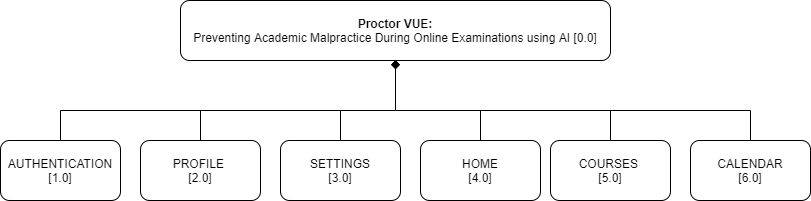
\includegraphics[scale=0.5]{main-hipo}
        \caption{Sample of HIPO}
    \end{center}
\end{figure}

\begin{figure}[h!]
    \begin{center}
        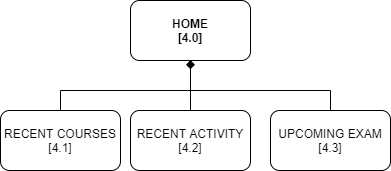
\includegraphics[scale=0.7]{home-hipo.png}
        \caption{Home Page}
    \end{center}
\end{figure}

\vspace{1cm}

\begin{figure}[h!]
    \begin{center}
        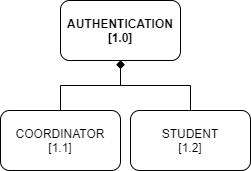
\includegraphics[scale=0.7]{auth-hipo.png}
        \caption{Authentication}
    \end{center}
\end{figure}

\begin{figure}[h!]
    \begin{center}
        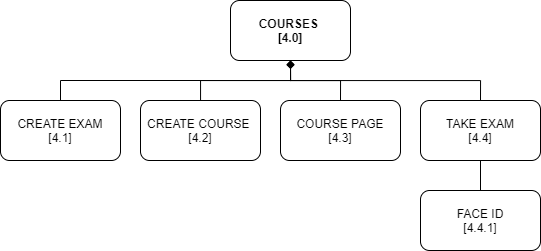
\includegraphics[scale=0.7]{courses-hipo.png}
        \caption{Courses}
    \end{center}
\end{figure}

\section{System Architecture}

\section{Conceptual Design}

\section{Cost Benefit Analysis}

\section{Requirement Analysis}

\section{Block Diagrams}

\section{Development and Testing}

\section{Input and Output Reports and Analysis}

\section{Description of the Prototype}

\section{Implementation Plan}

\section{Algorithm Use}

Proctor Vue utilizes an open source high-level face detection library, \lstinline{face-api.js}.
Under the hood, the library implements facial detection and recognition, as well as other useful functions such as age and gender recognition which are unused in Proctor Vue, using different machine learning algorithms to cater to different use cases.
The researchers wanted to have the most seamless and optimized experience during the exams so they opted to use the pre-trained tiny face detector model for the app's purposes.

The Tiny Face Detector model, unlike other well-known face detection models, is faster and more optimized, especially for detecting smaller faces out of a large image.
It makes intuitive use of different factors such as scale, resolution, and context for object detection.
In a research made by the original developers of the model, they found that the model can detect approximately 80\% of 1000 faces in a large image \cite{Hu_2017_CVPR}.

The facial recognition model, under the hood, is implemented using a residual network.
In practice, it will compute a descriptor for a person's face, describing their face's unique characteristics.
The model has an accuracy of 99.38\% in a facial recognition benchmark test.

\chapter{Recommendations}


\backmatter
\bibliographystyle{apacite}
\bibliography{references.bib}

\end{document}
